\documentclass[12pt,a4paper]{article}
\usepackage[T1]{fontenc}
\usepackage[utf8]{inputenc}
\usepackage{amsmath}
\usepackage{geometry}
\usepackage{graphicx}
\usepackage[colorlinks=true, linkcolor=black, urlcolor=blue]{hyperref}
\geometry{margin=1in}

\begin{document}
\pagenumbering{gobble}

\begin{titlepage}
    \centering

    {\Huge \textbf{Network Intrusion Detection with Classical Machine Learning}}\\[0.8cm]
    {\Large Project Report}\\[0.4cm]
    {\large Binary and Multiclass Classification on NSL-KDD}\\[3cm]

    {\large Hamza Abdelkader}\\[4cm]

    {\large \today}
\end{titlepage}

\clearpage
\pagenumbering{arabic}

\section{Introduction}

This project studies intrusion detection on the NSL-KDD dataset using a set of classical supervised learning models. NSL-KDD is a widely used benchmark for network security because it combines numerical and categorical features, strong class imbalance, and several attack families with very different frequencies.

The analysis covers two related tasks:
\begin{itemize}
    \item \textbf{Binary classification:} distinguish normal traffic from malicious traffic.
    \item \textbf{Multiclass classification:} predict one of five classes: Normal, DoS, Probe, R2L, or U2R.
\end{itemize}

Studying both settings makes it possible to compare how the same models behave when the output space becomes more complex. It also highlights how class imbalance affects evaluation, especially for rare categories such as R2L and U2R.

\section{Project Goals}

The main goals of the project are:
\begin{itemize}
    \item build a consistent preprocessing pipeline for mixed numerical and categorical data;
    \item compare several standard machine learning models on the same dataset;
    \item tune important hyperparameters with stratified cross-validation;
    \item evaluate generalization with accuracy, macro-F1, balanced accuracy, confusion matrices, ROC curves, and AUC;
    \item interpret the results through model assumptions, bias, variance, and class imbalance.
\end{itemize}

\section{Dataset}

The experiments use the NSL-KDD intrusion detection dataset, a refined version of the older KDD'99 benchmark. Each record describes a network connection through 41 features: 38 numerical attributes and 3 categorical attributes (\texttt{protocol\_type}, \texttt{service}, and \texttt{flag}).

Two label mappings were considered:
\begin{itemize}
    \item \textbf{Binary setup:} all attack types were merged into a single \textit{Attack} class.
    \item \textbf{Multiclass setup:} attacks were grouped into the standard families \textit{DoS}, \textit{Probe}, \textit{R2L}, and \textit{U2R}, with \textit{Normal} kept as a fifth class.
\end{itemize}

The binary training set contains 125{,}973 samples and the binary test set contains 22{,}544 samples. The multiclass problem is strongly imbalanced, which is especially visible for R2L and U2R.

\begin{figure}[htbp]
    \centering
    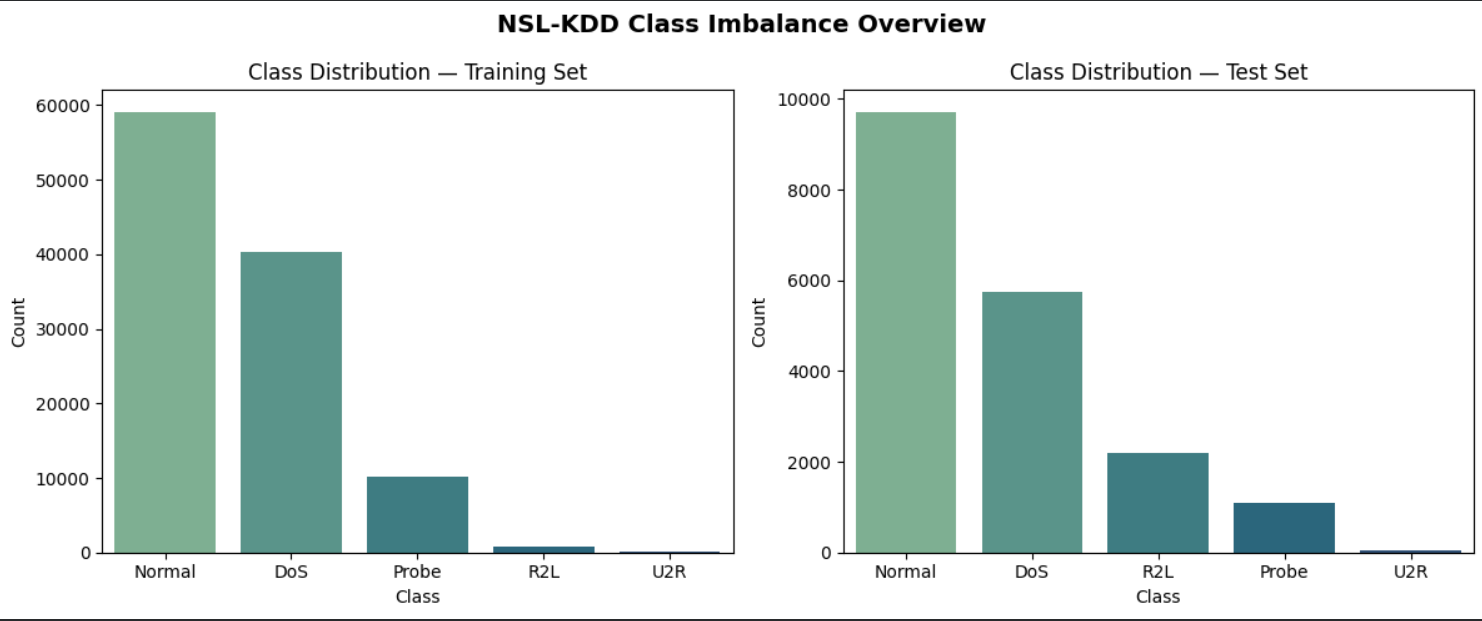
\includegraphics[width=0.9\textwidth]{class_distribution.png}
    \caption{Class distribution in the NSL-KDD training and test sets for the multiclass setting.}
    \label{fig:class_imbalance}
\end{figure}

No explicit rebalancing method such as oversampling, undersampling, or SMOTE was applied. This keeps the evaluation focused on how the models behave under the natural data distribution.

\section{Methodology}

\subsection{Preprocessing}

The preprocessing pipeline treats numerical and categorical features separately. Numerical features are standardized using
\[
z = \frac{x - \mu}{\sigma},
\]
while categorical features are one-hot encoded. The transformation is applied through a unified pipeline so that fitting happens only on the training split.

\begin{verbatim}
preprocessor = ColumnTransformer(
    transformers=[
        ("num", StandardScaler(), numeric_features),
        ("cat",
         OneHotEncoder(handle_unknown="ignore"),
         categorical_features)
    ]
)
\end{verbatim}

This design avoids data leakage, supports unseen categorical values at test time, and keeps the workflow reproducible.

\subsection{Models}

The following models were compared:
\begin{itemize}
    \item \textbf{Naive Bayes:} a probabilistic model with strong conditional independence assumptions.
    \item \textbf{Logistic Regression:} a linear classifier for the binary task.
    \item \textbf{Softmax Regression:} the multiclass extension of logistic regression.
    \item \textbf{Decision Tree:} a nonlinear classifier built from recursive impurity-based splits.
    \item \textbf{Random Forest:} an ensemble of decorrelated trees designed to reduce variance.
\end{itemize}

For the linear models, the decision rule is based on the logistic or softmax probabilities:
\[
P(y = 1 \mid x) = \sigma(w^\top x),
\]
\[
P(y = k \mid x) = \frac{\exp(w_k^\top x)}{\sum_j \exp(w_j^\top x)}.
\]

Decision Trees use impurity reduction, typically measured with the Gini index:
\[
G = \sum_k p_k (1 - p_k).
\]

\subsection{Model Selection and Evaluation}

Hyperparameters were tuned with 5-fold stratified cross-validation. This preserves class proportions across folds, which is especially important for the imbalanced multiclass task.

The evaluation emphasizes both overall performance and minority-class behavior:
\begin{itemize}
    \item accuracy;
    \item precision, recall, and F1-score;
    \item macro-F1;
    \item balanced accuracy;
    \item confusion matrices;
    \item ROC curves and AUC.
\end{itemize}

\section{Binary Classification Results}

\subsection{Cross-Validation and Test Accuracy}

\begin{table}[htbp]
\centering
\begin{tabular}{lcc}
\hline
\textbf{Model} & \textbf{Best CV Score} & \textbf{Test Accuracy} \\
\hline
Logistic Regression & 0.9965 & 0.7581 \\
Decision Tree       & 0.9993 & 0.7822 \\
Naive Bayes         & 0.9798 & 0.5646 \\
Random Forest       & 0.9999 & 0.7648 \\
\hline
\end{tabular}
\caption{Binary classification performance: cross-validation versus test accuracy.}
\end{table}

\noindent
\textbf{Observation:} cross-validation scores are extremely high for all models, especially the tree-based ones. The drop on the held-out test set suggests that the dataset is easy to fit in-sample but substantially harder to generalize on unseen traffic.

\subsection{ROC Curves}

\begin{figure}[htbp]
    \centering
    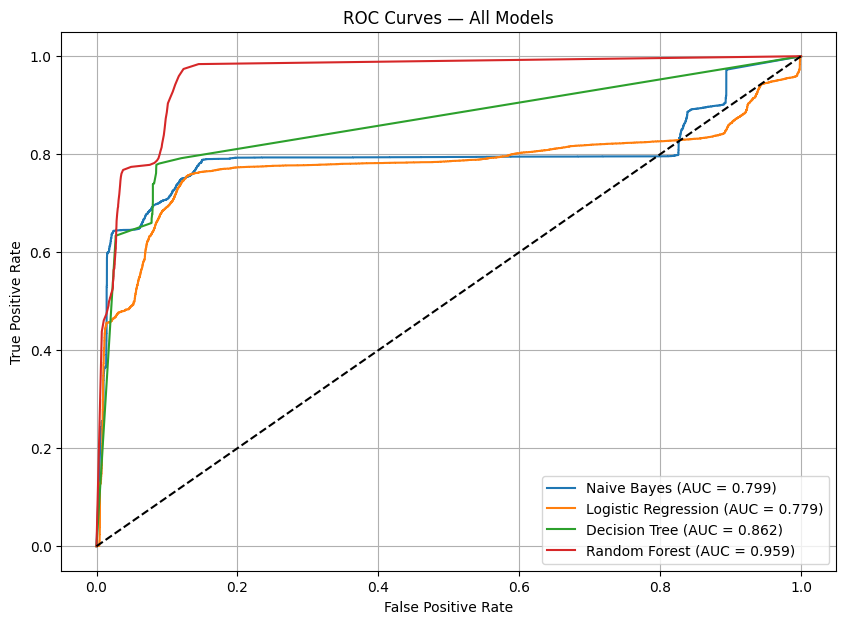
\includegraphics[width=0.85\textwidth]{binary_roc.png}
    \caption{ROC curves for the binary classification task.}
\end{figure}

Random Forest achieved the strongest binary ROC-AUC (0.959), followed by Decision Tree (0.862). The linear and probabilistic models showed weaker separation, which is consistent with their more restrictive assumptions.

\subsection{Confusion Matrices}

\begin{figure}[htbp]
    \centering
    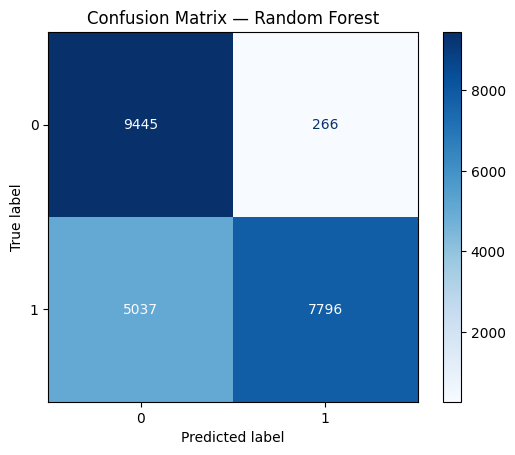
\includegraphics[width=0.42\textwidth]{binary_cm_rf.png}
    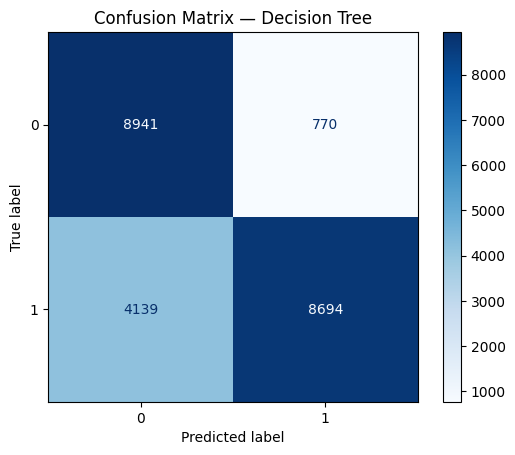
\includegraphics[width=0.42\textwidth]{binary_cm_dt.png}
    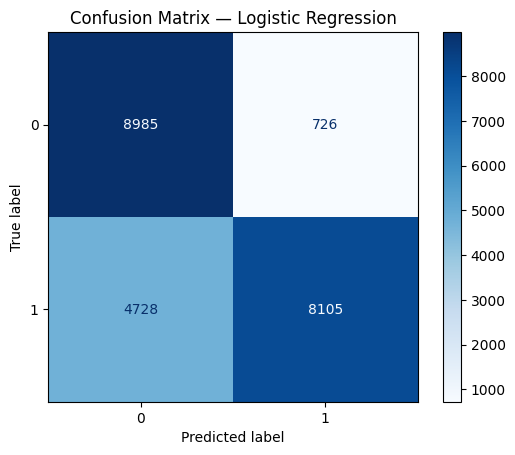
\includegraphics[width=0.42\textwidth]{binary_cm_lr.png}
    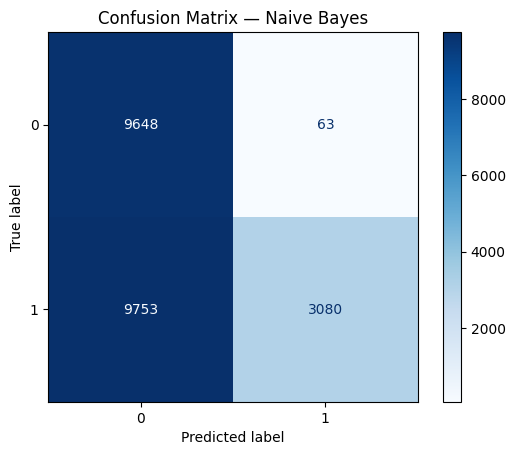
\includegraphics[width=0.42\textwidth]{binary_cm_nb.png}
    \caption{Confusion matrices for the binary classification task.}
\end{figure}

The confusion matrices show a clear ranking:
\begin{itemize}
    \item \textbf{Naive Bayes} overpredicts the majority pattern and struggles to balance false positives and false negatives.
    \item \textbf{Logistic Regression} offers a solid tradeoff and benefits from stable convex optimization.
    \item \textbf{Decision Tree} captures nonlinear interactions more effectively and reaches the best binary macro-F1.
    \item \textbf{Random Forest} provides the best probability ranking and the most balanced overall performance.
\end{itemize}

The reported binary macro-F1 scores are 0.76 for Logistic Regression, 0.78 for Decision Tree, 0.76 for Random Forest, and 0.52 for Naive Bayes.

\section{Multiclass Classification Results}

\subsection{Cross-Validation and Test Performance}

\begin{table}[htbp]
\centering
\resizebox{\textwidth}{!}{%
\begin{tabular}{lcccc}
\hline
\textbf{Model} & \textbf{CV F1 (macro)} & \textbf{Test Accuracy} & \textbf{Test F1 (macro)} & \textbf{Balanced Accuracy} \\
\hline
Naive Bayes        & 0.4333 & 0.5899 & 0.4097 & 0.5087 \\
Softmax Regression & 0.8581 & 0.8447 & 0.6499 & 0.6612 \\
Decision Tree      & 0.9068 & 0.8445 & 0.5941 & 0.6211 \\
Random Forest      & 0.9158 & 0.8803 & 0.6759 & 0.6765 \\
\hline
\end{tabular}%
}
\caption{Multiclass classification performance on the NSL-KDD test set.}
\end{table}

Random Forest produced the strongest multiclass results overall, while Softmax Regression remained highly competitive. The macro-F1 scores are more informative than accuracy here because they penalize failures on minority classes.

\subsection{ROC Curves}

\begin{figure}[htbp]
    \centering
    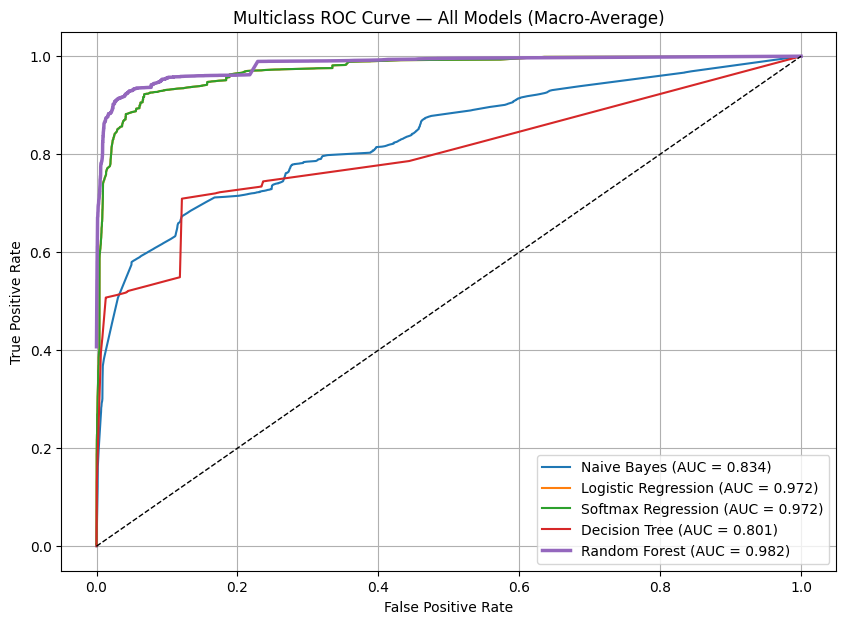
\includegraphics[width=0.9\textwidth]{multiclass_roc.png}
    \caption{Macro-averaged ROC curves for the multiclass classification task.}
\end{figure}

Random Forest achieved the strongest macro-averaged AUC (0.982), indicating the best overall class separation.

\subsection{Confusion Matrices}

\begin{figure}[htbp]
    \centering
    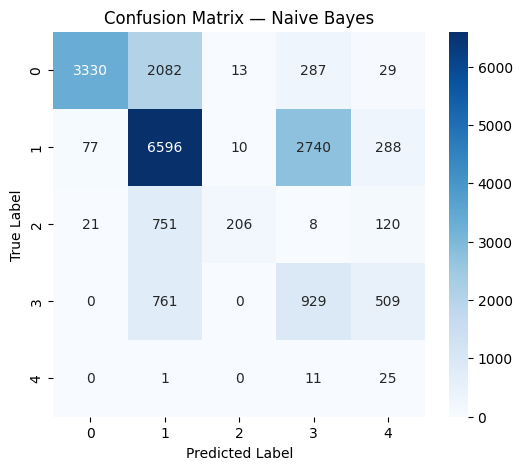
\includegraphics[width=0.42\textwidth]{mc_cm_nb.png}
    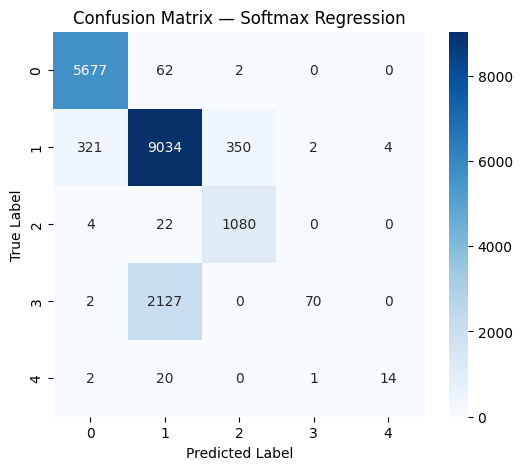
\includegraphics[width=0.42\textwidth]{mc_cm_softmax.png}
    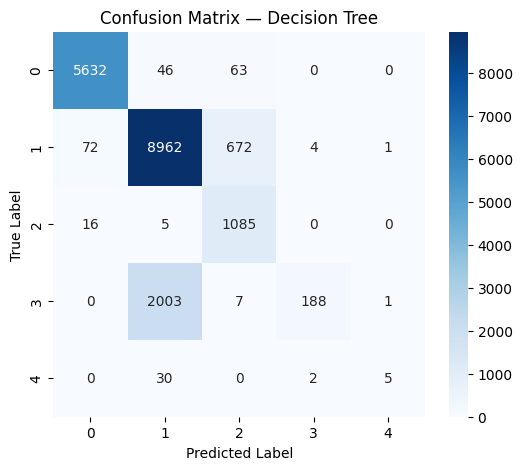
\includegraphics[width=0.42\textwidth]{mc_cm_dt.png}
    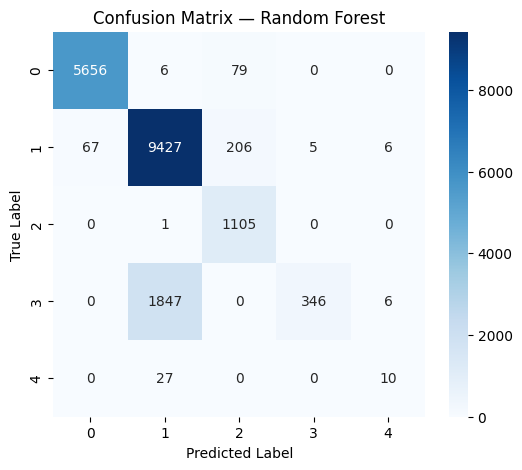
\includegraphics[width=0.42\textwidth]{mc_cm_rf.png}
    \caption{Confusion matrices for the multiclass classification task.}
\end{figure}

The confusion matrices reinforce the main challenges of the multiclass setting:
\begin{itemize}
    \item \textbf{Naive Bayes} performs poorly on overlapping and minority classes.
    \item \textbf{Softmax Regression} is stable and competitive but still struggles on rare classes.
    \item \textbf{Decision Tree} fits frequent classes well but loses robustness on minority categories.
    \item \textbf{Random Forest} provides the best overall robustness, though rare-class prediction remains difficult.
\end{itemize}

\section{Comparative Analysis}

\subsection{Binary vs. Multiclass Difficulty}

The binary task is substantially easier than the multiclass task. In the binary setup, most models achieve reasonable test accuracy because they only need to separate benign and malicious traffic. In the multiclass setup, the models must separate five classes simultaneously, including two extremely rare classes. This increases overlap, amplifies the effect of label imbalance, and makes evaluation much more sensitive to model assumptions.

\subsection{Effect of Model Assumptions}

Each model reflects a different bias--variance profile:
\begin{itemize}
    \item \textbf{Naive Bayes} has high bias and low variance. Its independence assumption is too restrictive for NSL-KDD, which explains its weak performance.
    \item \textbf{Logistic and Softmax Regression} have moderate bias and stable optimization. They work well when the transformed feature space is close to linearly separable, but they miss some nonlinear attack structure.
    \item \textbf{Decision Tree} has low bias but high variance. It can fit the training data extremely well and still generalize poorly.
    \item \textbf{Random Forest} reduces tree variance through bagging and random feature selection, which explains its superior overall performance on both tasks.
\end{itemize}

\subsection{Generalization}

The gap between cross-validation and test performance is especially informative for the tree-based methods. Decision Tree and Random Forest reach near-perfect cross-validation scores in the binary task and very high cross-validation macro-F1 in the multiclass task, but both decline on the held-out test set. This pattern strongly suggests overfitting pressure, even after hyperparameter tuning.

Softmax Regression shows a smaller generalization gap, which is consistent with its convex optimization and stronger regularization. Naive Bayes shows relatively smaller gaps as well, but mostly because its ceiling is already low.

\subsection{Class Imbalance}

Class imbalance is the defining difficulty of the multiclass problem. Accuracy alone hides the fact that most models struggle on R2L and U2R. Metrics such as macro-F1 and balanced accuracy make these weaknesses visible. Random Forest is the most robust model under imbalance, but even it does not fully solve the rare-class problem.

\section{Conclusion}

This project shows that classical machine learning models remain effective for tabular intrusion detection, especially when combined with careful preprocessing and cross-validation.

Random Forest emerged as the strongest model overall. It delivered the best binary ROC-AUC, the best multiclass accuracy, the best multiclass macro-F1, and the best balanced accuracy. Softmax Regression was also a strong baseline, particularly in the multiclass setting, thanks to its stable optimization and good generalization. Decision Trees worked well in the binary task but showed clearer signs of high variance. Naive Bayes underperformed consistently because its independence assumptions were too restrictive for this dataset.

Future improvements could focus on class-imbalance handling, cost-sensitive learning, threshold tuning, or more advanced ensemble methods. Even without those extensions, the current results provide a useful comparison of how standard models behave on a challenging intrusion-detection benchmark.

\end{document}
